\documentclass[Main]{subfiles}

\begin{document}

\chapter{Scope}

\section{Identification}
This System Requirement Specification (SRS) - Version 1.0 identifies, specifies and establishes the detailed system requirement for the Self Protection Suite as set forth by the Systems engineering exercises and teaching materials - version 1.4 \cite{SE-book}.
The SRS further specifies the methods to be used to ensure that each requirement has been met. 

\section{System overview}
The purpose of the SRS is to provide Royal Danish Air Force with a self-protection suite for the F-16 combat aircraft which will dispense payloads and host the MWS. 
The system will provide warning upon detection of missile threats and automatically dispense payloads in response.

\begin{figure}[H]
\centering
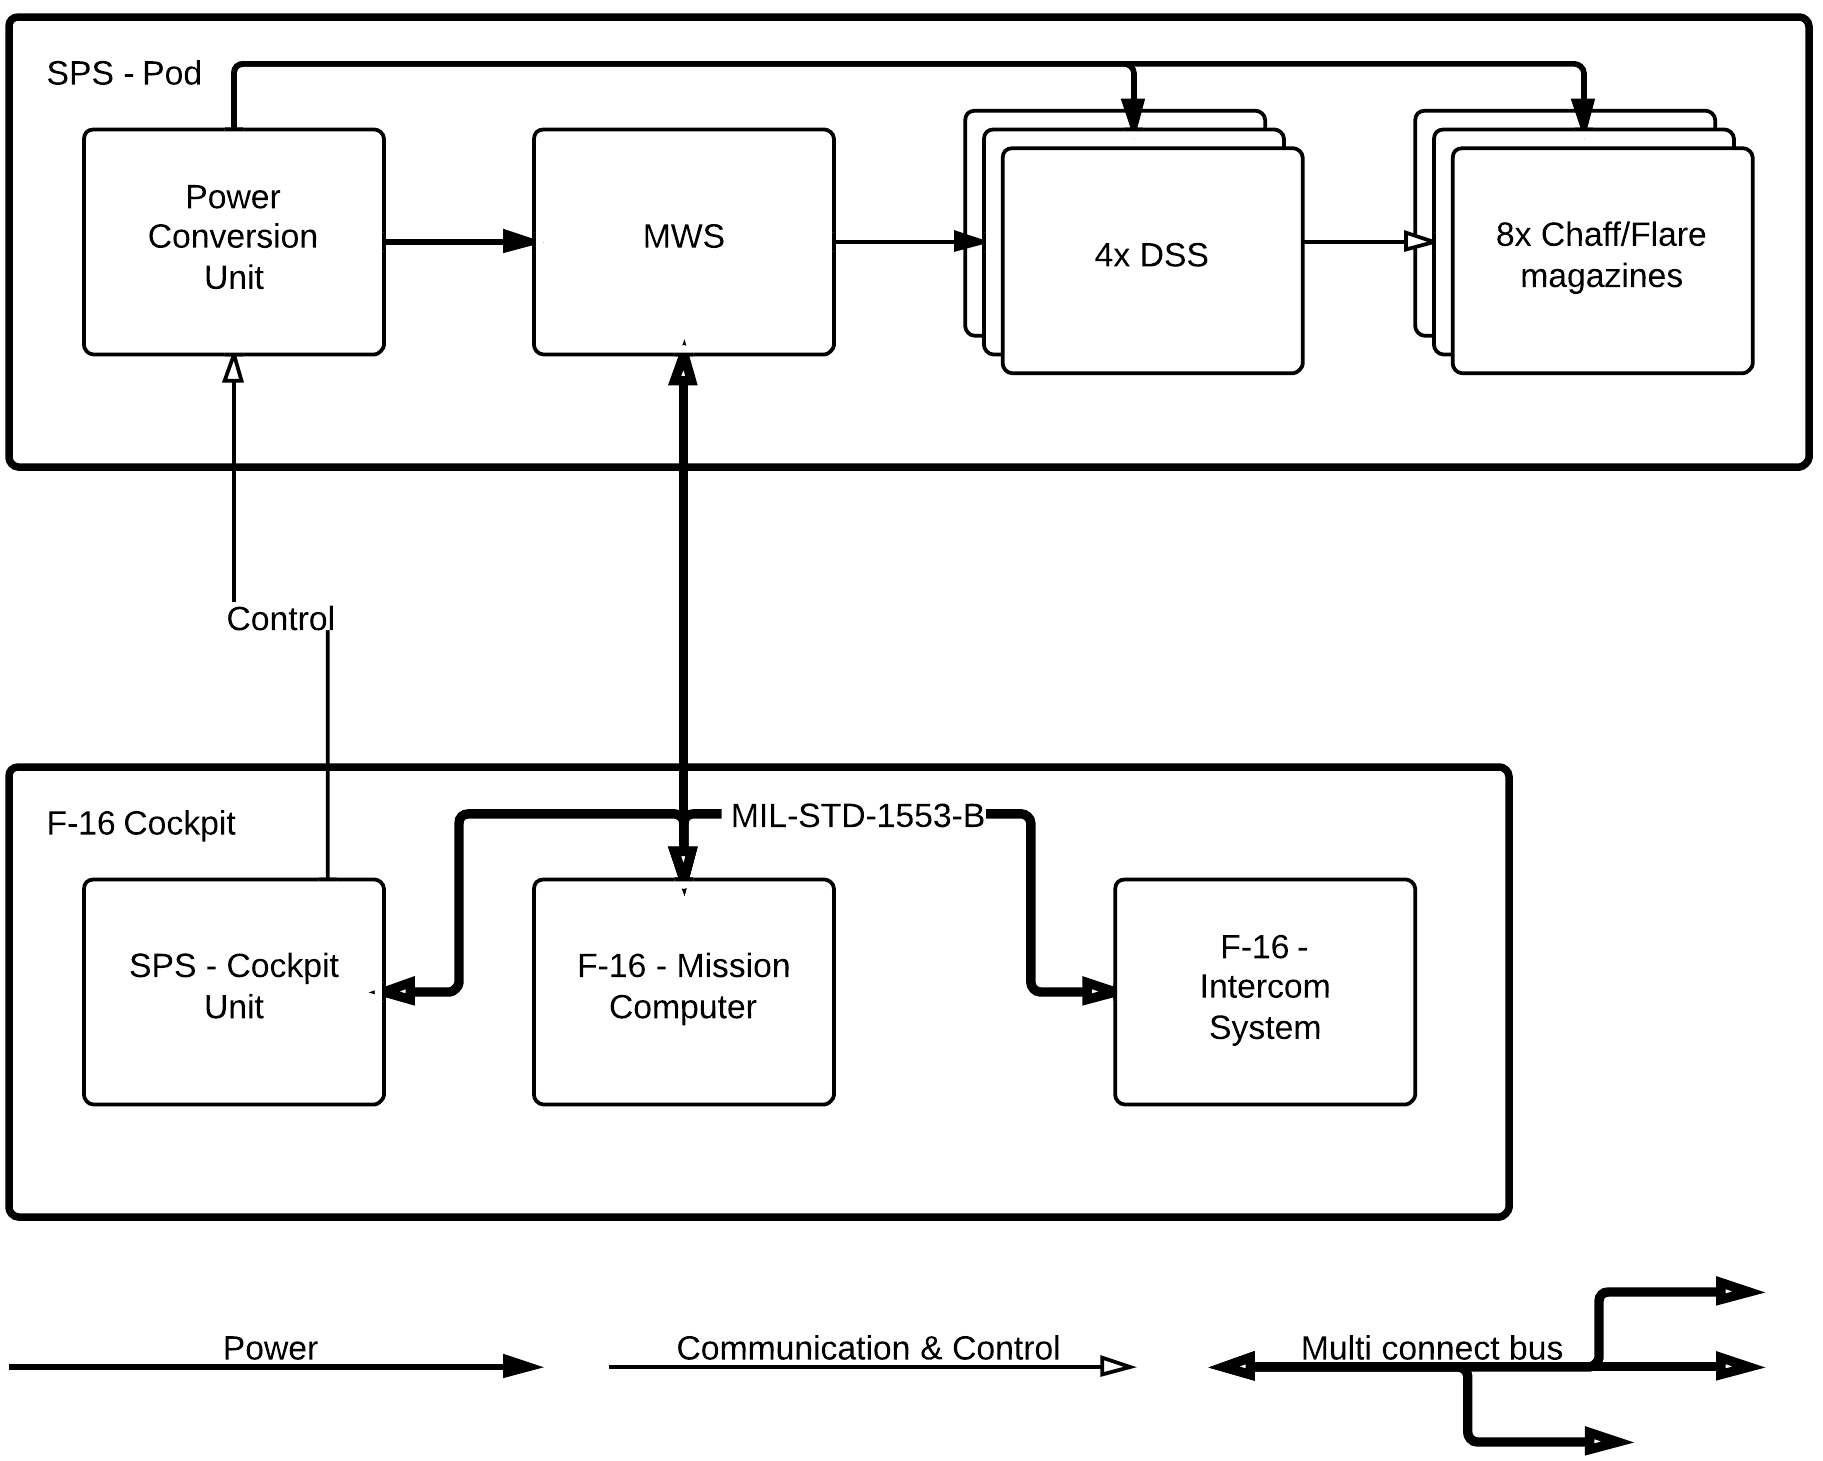
\includegraphics[width = 0.9\textwidth]{ConceptOfOperations}
\caption{Concept of operations}
\end{figure}


\section{Document overview}
This section has been tailored out. See Table of Contents.



\end{document}